% STM32Zombie-MS.tex
\begin{hcarentry}[new]{STM32-Zombie}
\report{Marc Fontaine}%11/17
\status{active}
\makeheader

%**<img width=700 src="./board3.jpg">
%*ignore
\begin{center}
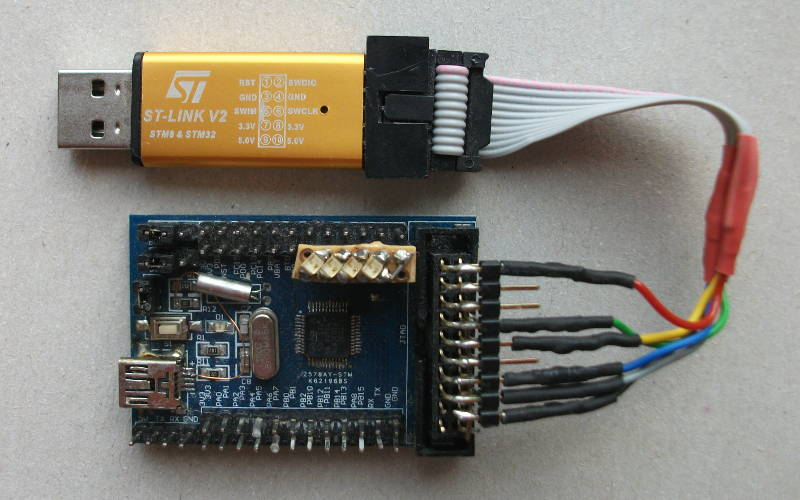
\includegraphics[width=.6\columnwidth]{html/board3.jpg}
\end{center}
%*endignore

The {\em STM32-Zombie} project turns a \texttt{STM32Fxxx} micro controller
into a Haskell programmable and flexible IO peripheral of your PC. The
\texttt{STM32Fxxx} micro controller family features a variety of powerful
\texttt{IO} peripherals like \texttt{GPIO} ports, \texttt{USART},
\texttt{SPI}, \texttt{I2C}, \texttt{USB}, \texttt{ADC}, timers, real time
clock, etc.\, and {\em STM32-Zombie} allows a Haskell program to control the
complete set of built-in micro controller peripherals.

The project is called {\em STM32-Zombie} because it shuts down the controllers
brain (the \texttt{ARM} \texttt{CPU}) and turns it into a remote controlled
zombie. It works without any c-code, cross-compiler tool-chain, or firmware.
The \texttt{STM32Fxxx} peripherals use memory mapped control registers and the
on-chip-debugging interface of the controller allows Haskell to access all of
the controllers address space and registers. With help of the \texttt{DMA}
controller even hard-real-time applications, like high-frequency sampling or
generating of high-frequency output patterns, are possible.

Minimal hardware requirements, for trying out this project, are a mini
\texttt{STM32F103} breakout board and a \texttt{STLink V2 USB dongle
simulator}. Both parts are available for less then \$2 each. My test setup are
mini \texttt{STM32F103} breakout boards. I have not tested the library with
other members of the \texttt{STM32Fxxx} family but the library is probably a
good starting point for work on other \texttt{STM32Fxxx} controllers.

The cabal package contains examples for LED blinking, serial port, SPI,
high-frequency ADC sampling, control of \texttt{WS1228B RGB LED} strips, and
more.

The library uses the naming conventions of the {\em ST-Microelectronics
STM32F10x Firmware Library} and provides a mid-level abstraction of the
hardware.

While access to all of the peripherals is possible, the abstraction layer is
still work-in-progress and does not cover all of the peripherals yet.

Comments, suggestions, experience reports, and patches are welcome. The
project is open to any kind of contribution.

\FurtherReading
  {\small
\begin{compactitem}
\item\url{https://github.com/MarcFontaine/stm32hs}
\item\url{http://hackage.haskell.org/package/STM32-Zombie}
\end{compactitem}
  }
\end{hcarentry}
